\documentclass[a4paper,11pt]{article}
\usepackage[osf]{mathpazo}
\usepackage{ms}
\usepackage[]{natbib}
\raggedright

\newcommand{\plant}{\texttt{plant}}
\newcommand{\smurl}[1]{{\footnotesize\url{#1}}}
\usepackage{graphicx}

\title{{\plant}: A package for modelling forest trait ecology \& evolution}
\author{Daniel S. Falster\textdagger\textasteriskcentered, Richard G. FitzJohn\textdagger, and Mark Westoby}
\affiliation{
Department of Biological Sciences, Macquarie University, Sydney, NSW 2109, Australia\\
\textdagger These authors contributed equally.\\
\textasteriskcentered Email for correspondence: \texttt{daniel.falster@mq.edu.au}\\
A manuscript in consideration as an Applications Note for
publication in MEE as part of the Special Feature \emph{Demography
  beyond the Population}.\\
Word count: ~3900 words}
\date{}

\bibliographystyle{mee}

\usepackage[title,titletoc,toc]{appendix}

\mstype{Applications Note}
\runninghead{The {\plant} package}
\keywords{demography, emergent, fitness, growth,
physiology, metapopulation, mortality, reproduction, size-structure,
tradeoff}

\begin{document}
\mstitlepage
\noindent
\parindent=1.5em
\addtolength{\parskip}{.3em}
\doublespacing
\linenumbers
\section{Summary}\label{abstract}
\begin{enumerate}
\def\labelenumi{\arabic{enumi}.}
\itemsep1pt\parskip0pt\parsep0pt
\item
  Population dynamics in forests are strongly size-structured:
  larger plants shade smaller plants while also expending
  proportionately more energy on building and maintaining woody stems.
  Although the importance of size-
  structure for demography is widely recognised, many mechanistic models
  either omit it entirely, or include only coarse approximations.
\item
  Here we introduce the {\plant} package, an
  extensible framework for modelling size- and trait-based demography,
  ecology and evolution in simulated forests.
  At its core, {\plant} is an
  individual-based mechanistic model where plant physiology and demography are mediated by
  traits. Individuals from multiple species can be grown in isolation,
  in patches of competing plants, or in metapopulations under a
  disturbance regime. Dynamics within patches of competing plants can be
  resolved either in a stochastic, finite-sized patch; or deterministically, using
  novel extensions of the ``Escalator Boxcar Train''
  technique. Combined effects of trait-, size- and patch-structured
  dynamics are integrated into metapopulation level estimates of
  invasion fitness and vegetation structure. Since fitness emerges as a
  function of traits and is integrated over a full metapopulation, plant
  provides a novel arena for exploring eco-evolutionary dynamics.
\item
  {\plant} is an open source R package and is available at
  \href{https://github.com/traitecoevo/plant}{github.com/traitecoevo/plant}.
  While accessed from R, the core routines in {\plant} are written in C++.
  The package provides for alternative physiologies and for
  hyper-parameterisation to capture trade-offs among parameters. A
  detailed test suite is provided to ensure correct behaviour of the code.
\item
  {\plant} provides a transparent platform for investigating how
  physiological rules and functional trade-offs interact with competition and
  disturbance regimes to influence vegetation demography, structure and
  diversity.
\end{enumerate}

\section{Introduction}\label{introduction}

Plant growth and demography are fundamentally size- and
trait-structured, influencing dynamics over time-scales ranging from
instantaneous physiological effects to long-term evolutionary outcomes
\citep{Harper-1977, Westoby-2002}.
%
As an individual increases its leaf area, it increases its potential
to generate photosynthate.
%
On the other hand as individuals grow larger they must allocate increasing
fractions of their photosynthetic income to activities other
than building new leaves; for example, to maintaining support tissues
\citep{Givnish-1988, Enquist-2007} or to reproduction
\citep{Thomas-2011}.
%
Consequently rates of growth, mortality and reproduction change with
individual size \citep{Muller-2006, Ruger-2011, Thomas-2011}.
Ontogenetic
patterns of growth also vary with traits; for example,
leaf and wood construction costs influence growth rates
\citep{Wright-2010}, while seed size and height
at maturation determine the start and end points of ontogenetic
trajectories \citep{Westoby-2002}.
%
Strong feedbacks emerge between individuals within a forest via
competition for light and other resources, such that the growth rate
of one individual depends on the size and traits of nearby
individuals \citep{Shugart-1980, Pacala-1996}.
%
Such feedbacks make it difficult to link observable species traits to
phenomena such as self-thinning, successional transitions, trait
evolution and species coexistence, without
modelling both individual growth and the competitive interactions between
individuals.

Although the importance of size-structure for trait evolution, vegetation
dynamics and diversity has been long been recognised \citep[e.g.,][]{Harper-1977,
  Shugart-1980, Huston-1987}, current research in this area is
dominated by models and theory that either omit size-structure
entirely, or only include coarse approximations.
%
Theoretical investigations exploring questions about niche-based
species coexistence and ecological drift (neutrality) both rely
primarily on unstructured population models \citep[e.g.][]{MacArthur-1967,
  Tilman-1985, Geritz-1998, Hubbell-2001, Calcagno-2006}.
%
It is common to assume competitive outcomes are influenced by
size-related traits such as adult and seed size, but detailed
size-structure is rarely considered, at least in plant models
\cite[for animal examples, see][]{Deroos-1988, Deroos-1992}.
%
Similarly, many of the models used to study global vegetation dynamics across
the last 20 years have not included size-structured demography
\citep[for comparisons of some major models see][]{Sitch-2008,
Dekauwe-2014}.
%
While the importance of explicitly including size-structured dynamics is
increasingly recognised in both areas of evolutionary ecology
\citep[e.g.][]{Falster-2015} and vegetation dynamics
\citep[e.g.][]{Moorcroft-2001, Purves-2008, Smith-2014,
Weng-2015, Sakschewski-2015}, our understanding on how these features
impact on the ecology and evolution of vegetation communities remains
relatively limited.

In this note, we introduce the {\plant} package for R \citep{R-2015};
a mechanistic framework for studying the effects of size structure and
trait variation on the demography of individual plants, of patches of
competing plants and of meta-populations structured by a prevailing
disturbance regime.
%
Our own purpose in developing {\plant} has been mainly to investigate how species
differing in traits may be able to coexist with one another
\citep[following ][]{Falster-2011, Falster-2015}; as size-structured models
provide unique opportunities for studying coexistence via differentiation in
successional strategy \citep[see also][]{Huston-1987, Moorcroft-2001}.
At the same time, we expect {\plant} to be useful for modelling other demographic phenomena.

Broadly, the {\plant} model falls into a class we refer to as Trait- Size- and
Patch- structured Models \citep[\textsc{TSPMs}, following][]{Falster-2011}. \textsc{TSPMs} are direct
descendants from the ``gap'' models developed in 1980s
\citep[e.g.][]{Shugart-1980, Huston-1987, Kohyama-1993}; other modern examples
include \textsc{ED} \citep{Moorcroft-2001}, \textsc{LPJ- GUESS}
\citep{Smith-2014} and \textsc{LPJml-FIT} \citep{Sakschewski-2015}. Common to
\textsc{TSPMs} is that they explicitly model size-structured competition
among individual plants within a metapopulation of ``patches'', where
individuals can also differ in their traits and thus demographic behaviour.
\textsc {TSPMs} typically ignore the spatial structure of plants within
patches and the spatial structure of patches relative to one another. Instead
they focus computational effort on resolving the dynamics of size-structured
competition for light and successional turnover. Differences among
\textsc{TSPMs} arise from the core physiological models used (describing
how the demography of individual plants responds to resource availability),
and also from the numerical techniques applied to scaling the physiological model up to
estimate emergent behaviours of individuals, patches and vegetation.

Below we describe the general approach of the package, then provide
sections outlining potential applications at nested levels of ecological organisation.
Detailed technical documents are provided as supplementary information
(see Appendices); updated versions of these technical documents are
available within the {\plant} package itself.

\section{Overview of approach}

{\plant} is an individual-based model, meaning the dynamics of the
population arise from rules specifying how individuals grow and interact.
Being driven by traits, the model can be extended to potentially very many species. The
core rules in {\plant} are about the short-term physiological
functioning of an individual plant and how this is influenced by its
traits, size and light environment.  While {\plant} includes a core physiological model, the present paper does not aim to justify the particular physiological model used, to provide detailed
comparisons to data, or to promote this physiological model over those in other \textsc{TSPMs}. (These are all topics deserving substantially more attention than can be afforded here.) An important feature of {\plant} considered as a software package is that it allows for users to substitute their own physiological models.

On top of the physiological model, {\plant} implements methods for
population and adaptive dynamics (Fig.  \ref{fig:schematic}) following methods
described by \citet{Falster-2011} and \citet{Falster-2015}. Demographic
phenomena can be studied at the three levels: individual plants, stands of
competing plants and entire metapopulations. The dynamics at these higher
levels of organisation arise as emergent properties, driven by growth
physiology, competition for light and disturbance (Fig.  \ref{fig:schematic}).
{\plant} offers the capacity to model emergent behaviour of patches with
specified size, and also a deterministic size-independent approximation
where specifying a patch size is not required. Trait evolution and community
assembly can then be modelled using the estimates of invasion fitness
provided by {\plant}.

\section{Effects of size, trait and environment on demography of individual plants}

The core of {\plant} is a model for an individual species' physiological
strategy as specified by its traits (Fig. \ref{fig:schematic}a). For
present purposes, a species is defined as a group of individuals with identical
traits. The effects of trait variation is to modify parameters of the core
physiological model, which in turn translate into different demographic outcomes.

The default physiological model used in {\plant} largely reflects
that presented in \citet{Falster-2011,Falster-2015}, but with extensions
allowing for diameter growth also to be estimated. We refer to this
default model as \texttt{FFW16}, reflecting the author's initials and
publication year of this paper. The \texttt{FFW16} model estimates rate
of biomass
production for a plant, given its size and the current light
environment. Gross photosynthetic income is calculated from the total
leaf area and the light distribution across the plant's canopy. Costs
of tissue respiration and turnover are then subtracted. The remaining
biomass production is then allocated between growth and reproduction. The key
outputs needed by higher levels of {\plant} are height
growth rate, mortality rate and rate of seed production.  However
additional quantities are also computed, such as total assimilation
and the respiration, turnover and allocation rates for different
tissues, and these intermediates can also be accessed (for further details on the \texttt{FFW16} model see Appendix
\ref{sec:plant}).

While we have implemented a particular physiological model (\texttt{FFW16}), the
package is designed to allow arbitrary additional physiologies to be
introduced. Users are able to modify the physiological model in two
different ways. First, one can vary the parameters of the \texttt{FFW16} model
directly (see Table XXX for list, for examples see Appendix
\ref{sec:parameters}). Second, we allow for changes in key parameters to
bring about changes in other parameters (a hyper-parameterisation), enabling
straightforward modelling of trade-offs. For example, the trait \textsc{lma}
(leaf mass per unit leaf area) is used to estimate the rate of leaf turnover
($k_l$), based on an observed scaling relationship spanning across diverse
vegetation and plant functional types \citep{Wright-2004}:
$$k_l = \beta_{kl1} \, \left(\frac{\phi}{\phi_0}\right)^{-\beta_{kl2}},$$
where $k_l$ and $\phi$ (lma) are both parameters of the core physiological
model, and $\beta_{kl1}, \beta_{kl2}, \phi_0$ are hyper-parameters. Such
linkages are defined within a user-supplied hyper-parameterisation function
(see Appendix \ref{sec:FFW16} for details). Finally, rather than varying the
parameters of the existing equations in the \texttt{FFW16} model, the
equations themselves can be changed and the higher level functionality of the
package can still be used.  Changed equations would amount to defining a new
physiological model in a new C++ file. As an example, in
the \texttt{FFW16b} physiology, we have modified the function determining
allocation to reproduction.

With a basic physiological model in place, {\plant} can be used to estimate
essential physiological rates for individual plants
(Fig. \ref{fig:plant}). The function \texttt{grow\_plant\_to\_size}
takes a given strategy and light environment and grows the plant,
producing a trajectory of size over time (Fig. \ref{fig:plant}a). This
is achieved by integrating an ordinary differential equation of
size-dependent growth rate (see Appendices \ref{sec:demography} and
\ref{sec:plant} for more details). As the plant grows, allocation to
different tissue types varies and the composition of the plant
changes to include more stem and less leaf
(Fig. \ref{fig:plant}b). This in turn affects maintenance and turnover
costs and the growth rate of the plant (Fig. \ref{fig:plant}c).  This
shift in allocation by itself can generate the widely-observed hump-shaped pattern
of absolute height growth with size \citep{King-2011} and the decline in relative mass growth rate with size from birth onwards \citep{Enquist-2007}.

By varying the light environment and measuring growth rate, the whole-plant light compensation point (\textsc{wplcp}) can be computed (Fig.
\ref{fig:plant}d). The \textsc{wplcp} is the light level at which the plant
stops growing and is increasingly regarded as the most useful
measure of a species' shade tolerance
\citep{Givnish-1988, Baltzer-2007, Lusk-2013}. As expected, \textsc{wplcp}
increases with plant size, due to increased costs of building and
maintaining stem and leaf tissues \citep{Givnish-1988}. Likewise, \textsc{wplcp}
decreases with \textsc{lma}, because high \textsc{lma} species have slower leaf turnover
\citep{Baltzer-2007, Lusk-2013} (Fig.
\ref{fig:plant}d).

\section{Plants competing in a patch}

Within patches of competing plants, competition for light generates
strong non-linear feedbacks on growth, survival and reproduction. In the
\texttt{FFW16} physiological model, we consider only the effect of
shading on rates of biomass production, although competition for other
resources such as nitrogen or water could also be considered by extending the
physiological model. We assume that patches are vertically but not horizontally
structured; in other words, we account for size differences but not spatial
layout within the patch. Similar assumptions are found in other \textsc{TSPMs}
\citep{Shugart-1980, Kohyama-1993, Huston-1987, Moorcroft-2001, Smith-2014}.
While ideally one would also consider spatial interactions within patches,
such models are very computationally demanding and also
impossible to solve in a deterministic fashion \citep{Shugart-1980,
Pacala-1996}. Moreover, it remains unclear whether resolving spatial details within a
patch would provide further useful ecological detail, in part because the
process of competitive thinning tends to break down spatial clusters
\citep{Strigul-2008}.

When modelling a patch of competing plants, the focus is on changes to the size-
density-distribution \(N(x, H, a)\) with patch age \(a\), i.e. the density of
individuals with traits \(x\) and height \(H\) within a patch of age \(a\).
Density is measured as individuals per unit height and per unit ground area.
Modelling the development of  \(N(x, H, a)\) requires that both the initial size
distribution and the inflow of new recruits be specified. We have primarily
been interested in dynamics of a patch recovering from disturbance and have
therefore started with an empty patch and constant flow of seeds from a global
seed rain (Fig. \ref{fig:schematic}b). A non-trivial extension could be added to allow some plants to survive disturbance \citep[following][]{Kohyama-1993}.

The {\plant} model offers two methods for modelling the dynamics of \(N(x,
H, a)\) in a competing population. In the first ``stochastic'' mode, users
specify an average seed rain and patch size, and {\plant} then generates a
vector of seed arrival events and simulates stochastic
development of the resulting finite-sized population (see Appendices XXX for an
example).

For most applications, however, rather than modelling
dynamics within a finite-sized stochastic patch, it will be preferable to use {\plant}'s
``deterministic'' approximation. The deterministic mode assumes that
patches are very large, so that the population dynamics within the
patch approach their deterministic limit and can
be approximated via a Partial Differential Equation (\textsc{pde})
\citep{Deroos-1997, Kohyama-1993}.  The same \textsc{pde} is also thought to
capture the average behaviour across a large number of small patches
\citep{Moorcroft-2001}. Importantly, the ``deterministic'' mode is
much faster than the stochastic model and without noise (more
details in Appendix \ref{sec:demography}).

Our approach for modelling deterministic size-structured population dynamics is
based on the Escalator Boxcar Train (\textsc{ebt}) technique
\citep{Deroos-1988, Deroos-1992, Deroos-1997, Brannstrom-2013}. The \textsc{ebt} solves
the \textsc{pde} describing development of \(N\) by approximating the
density function with a collection of cohorts spanning the size
spectrum. Following a disturbance, a series of cohorts are introduced
into each patch. These cohorts are then transported along the
characteristic equations of the \textsc{pde}. Biologically these are
the growth trajectories of individuals, conditioned on them surviving
(e.g. Fig. \ref{fig:patch}a). Meanwhile, growth and mortality combine
to alter the density of individuals along the trajectories
(Fig. \ref{fig:patch}b).

We introduce two extensions to the \textsc{ebt}: i) a new method for
estimating the size-density distribution and ii) a technique for
handling strong size-asymmetric competitive feedbacks, such as occur
under strong competition for light (see Appendix \ref{sec:demography}
for details). The original \textsc{ebt} proceeds by approximating the
first and second moments of the density distribution \(N\) within each
cohort \citep{Deroos-1997}.
%
In {\plant} we use a different approach. Instead of tracking first and
second moments of the size-distribution within cohorts, we track a
point mass estimate of \(N\) along the trajectory for the boundary of
each cohort. We found this approach preferable because it does not
require us to maintain a separate set of equations for the smallest
cohort.

The extension for handling strong size-asymmetric competition involves
adaptive refining of time points at which new cohorts are introduced
into the population, an idea first applied in \citet{Falster-2011} and
described further in \citet{Falster-2015}.
In the original \textsc{ebt}, cohorts were introduced at a fixed time
interval. Under competition, however, the growth
trajectories of individuals born at similar times can diverge
substantially over time (Fig. \ref{fig:patch}a; Appendix
\ref{sec:demography}, \ref{sec:cohort-spacing} and
\ref{sec:patch}). This can become a problem later during patch
development because much of the population can be located between
widely-spaced cohorts, causing low numerical accuracy. To maintain
numerical accuracy, we use an iterative algorithm to adaptively refine
the cohort spacing until the trajectories of adjacent cohorts remain
adequately resolved throughout development of the patch (see Appendix
\ref{sec:demography} for details). This refinement gives rise to uneven
distribution of cohort introduction times across patch age (Fig.
\ref{fig:patch}a), with considerably tighter spacing of cohorts in
younger patches.

Modelling of size-structured dynamics via solving a deterministic
\textsc{pde} enables multiple demographic phenomena to be
investigated. First, {\plant} can simulate demographic
phenomena typically observed in patches
recovering from a disturbance, including self-thinning and
successional replacement. Whereas other approaches for modelling
self-thinning are limited to a single species
\citep[e.g.][]{Barnes-2004, Coomes-2007}, \textsc{TSPMs} can accommodate
multiple species with different traits (Fig. \ref{fig:schematic}b;
Fig.  \ref{fig:patch}). Second, the self-thinning and
successional replacement emerge from the
combined effects of physiology and competition for resources, rather
than being prescribed in the model. As a consequence, it is possible to ask how alternative trait values would translate into demographic fitness (see further below). Third,  \textsc{TSPMs} allows for the combined effects of physiology and succession on emergent
characteristics of the entire patch to be investigated
\citep{Moorcroft-2001, Falster-2011}. Leaf area cover and rates of biomass
production tend to vary  non-linearly with patch
age \citep{Smith-2001, Binkley-2002, Ogawa-2010};
in {\plant} such outcomes arise naturally as emergent properties,
driven by demography (Fig. \ref{fig:patch}c).

\section{Trait, size and patch structured vegetation}

All vegetation in {\plant} is subject to a disturbance regime, such that patches
of the landscape are cleared at some rate, by fire, cyclone or
landslide.  The vegetation thus comprises a series of patches
differing in time since last disturbance and linked via seed dispersal
(Fig.  \ref{fig:schematic}b). Such a system is often referred to as a
structured metapopulation \citep{Gyllenberg-2001}.

In {\plant} and following \citep{Kohyama-1993, Moorcroft-2001,
  Falster-2011} we assume an infinite number of patches, all experiencing
the same disturbance regime and sharing a common seed dispersal pool
(i.e., the island model; Fig. \ref{fig:schematic}b). We also assume
that the disturbances remove all established vegetation.  With this
approach we can scale up from deterministically solving the dynamics of
a single patch to solving the dynamics of an entire metapopulation.
The frequency-density \(P(a)\) of patches aged
\(a\) in the landscape is needed. Assuming there are a large number of
patches means the dynamics of \(P\) behave deterministically and can
be approximated via a second \textsc{pde} (see Appendix
\ref{sec:demography} for details). Scaling from patch to
metapopulation is then achieved by weighting the temporal dynamics of
a single patch by \(P(a)\), the relative abundance of patches aged
\(a\) in the metapopulation (Fig. \ref{fig:patch}c).

The main numerical challenge in stepping from a single patch to a
metapopulation is to identify the equilibrium seed rain of the
metapopulation. An ``input'' seed rain is required to simulate the
demography of the metapopulation, and this in turn produces an ``output''
number of seeds. Equilibrium occurs when, for each species,
a given input seed rain produces an equivalent output seed rain. Finding this equilibrium
requires finding the root of a multi-dimensional function, subject to
the constraint that this root is stable (the trivial equilibrium
of zero seed rain always exists, but is often not stable; Appendix
\ref{sec:equilibrium}).  Real seed rains are of course quite noisy,
but this approach still allows for the mean tendencies to be estimated.

An attractive feature of the metapopulation concept implemented in \textsc{TSPMs}
is that integrates both equilibrium and non-equilibrium approaches to
modelling ecological dynamics \citep{Kohyama-1993, Moorcroft-2001,
  Falster-2011}. An equilibrium may be approached at the level of
metapopulation, meaning the seed rain and size structure across the
entire metapopulation is approximately stable. Yet the structure of
vegetation within individual patches is constantly in flux. Patches
continue to age and their residents continue to grow until they are
disturbed.

The dynamic equilibrium captured by the trait-, size- and
patch-structured metapopulation model potentially resolves several
challenges faced by unstructured models. First, by scaling up from
patch to metapopulation, we close the demographic feedback loop to
create a self-regulating system. The equilibrium seed rains and size-density distributions  arise for each species present as outputs from the model, based on the combined effects of the model's physiological rules, species traits, competitive interactions
and the prevailing disturbance regime.

Second, the metapopulation concept allows for the effects of disturbance
regimes on vegetation structure and dynamics to be properly incorporated. In
{\plant} characteristics for the entire vegetation (metapopulation) -- such
as total leaf area, biomass and productivity -- are obtained by averaging
patch-level outcomes over the frequency-distribution of patch ages (e.g.
Fig. \ref{fig:patch}c).  Similarly, the distributions of  abundance and growth rate
observed in large forest  plots \citep[e.g.][]{Muller-2006, Coomes-2007} arise
as  emergent phenomena. Moreover, the predictions from {\plant}
are for a frequency distribution of patch states across the landscape
(Fig. \ref{fig:emergent}, see more detail in Appendix \ref{sec:emergent}). As such,
size- and patch-structured models provide unique opportunities for linking with
satellite and forest survey data \citep{Moorcroft-2001, Purves-2008}.

Finally, with the extension to the metapopulation level, we are
modelling demography across the entire life cycle and are thus in a
position to estimate invasion fitness -- the ability of a rare
individual with particular traits to establish in a community of
established residents at their equilibrium densities
\citep{Metz-1992, Chesson-2000}.  While ideally calculated as the
long-term per capita growth rate, a more convenient indicator of
fitness in structured metapopulations is given by the
logarithm of the basic reproduction ratio, \(R\) \citep{Gyllenberg-2001, Metz-2001}. The basic reproduction ratio is simply the average number of seeds produced from one seed of a new type over its lifetime, averaged across the metapopulation. So a new type can
invade when \(\log R > 0\).

With this measure of fitness, we can model trait-based adaptive
dynamics and community assembly of forest communities, following
 \citep{Falster-2015}. This is best thought of as occurring on a fitness landscape, a surface with fitness plotted against one or more species traits
(Fig. \ref{fig:fitness}). The reproductive success of individuals
depends both on their own traits and on densities of other occupants in the current resident community. Fitness landscapes will be positive in regions that allow invasion, and zero
for species that are at equilibrium. The slope of the fitness
landscape with respect to traits indicates the direction of selection
(dashed line in Fig. \ref{fig:fitness}a) indicates selection for
smaller trait values (see Appendix \ref{sec:fitness} for
details)). Fitness landscapes are continually reshaped as species are
introduced and their trait values evolve, reflecting the non-linear demographic feedbacks
that occur under frequency-dependent evolution. Stable coexistence is
possible when species with different traits can mutually invade
\citep{Geritz-1998, Chesson-2000}. Following the fitness gradient may lead to an
evolutionary branching point \citep{Geritz-1998}; at
such a point there is no directional selection (solid line in
Fig. \ref{fig:fitness}a) but invasion is possible both above and below
it in trait space. It is often possible to find a configuration where
fitness is negative everywhere (solid line in Fig. \ref{fig:fitness}b)
except for the zero points where species are present. This community
is immune to invasion from any other strategies and represents a
prediction for the trait mixture that might be favoured by
natural selection \citep{Geritz-1998}.

In general,  a variety of algorithms from the area of adaptive dynamics could be applied for modelling community assembly \citep[e.g.][]{Geritz-1998, Falster-2015}, using the estimate of invasion fitness provided by {\plant}.

Identifying conditions promoting trait diversity is a valuable role
for {\plant}. The simple example here can be extended to multiple dimensions
and can be used to investigate how trade-offs facilitate coexistence
\citep{Falster-2015}. Co-occurring plant species differ in a range of physiological
traits, yet the conditions allowing for stable coexistence remain largely
unknown \citep{Adler-2013}.

\section{Implementation details}

{\plant} is written in C++ and R, using the package \texttt{Rcpp}
\citep{Eddelbuettel-2011, Eddelbuettel-2013} to bridge between the two
languages. Due to the computationally intensive nature of the model,
the core physiological and demographic components are in C++ to
maximise speed. We used templated types that allow the demographic and
evolutionary components to be driven by alternative physiological
models while retaining the same interface at higher levels. Despite
mostly being written in C++, all components of the model, down to
individual plants, can be extracted and interacted with dynamically in
R, using the \texttt{RcppR6} package \citep{RcppR6}.

{\plant} makes use of much existing software, including the R
computational environment \citep{R-2015}, the R packages \texttt{Rcpp}
\citep{Eddelbuettel-2011, Eddelbuettel-2013}, \texttt{R6}
\citep{Chang-2014}; and the Boost Library for C++
\citep{Schaling-2014} via the R package \texttt{BH}
\citep{Eddelbuettel-2015}. Source code is hosted at
\href{https://github.com/traitecoevo/plant}{github.com/traitecoevo/plant}.
Installation instructions are available at this webpage, binary
releases will also be available there.  {\plant} does not
currently compile on Windows, but this will change as soon as R core
upgrade the Windows C++ compiler).

\section{Comparison to existing software}

Increased interest in capturing the behaviour of size-structured  populations
has prompted development of several tools, each with its own distinct
strengths. The \textsc{EBT} software (see De Roos XXXX in this special feature) provides
a flexible framework that has been used to study a range of marine organisms.
Compared to the \textsc{EBT}, {\plant} is more focussed on plants, and
to that end offers refinements needed to handle modelling of the strong
size-asymmetric feedbacks that occur in plant communities, as well as the
extension to structured metapopulation. Other \textsc{TSPMs} also exist for modelling of vegetation, like \textsc{ED}
\citep[ver 1 and 2][]{Moorcroft-2001, Medvigy-2009}, \textsc {LPJ-GUESS}
\citep{Smith-2014} and a\textsc{LPJml-FIT}  \citep{Sakschewski-2015}. These
models were designed for simulation of bio-geochemical cycles and vegetation
structure across broad geographic areas, and their architectures are
optimised for such use. By contrast, {\plant} was  designed so that the
physiological rules driving the dynamics of the system could be easily
manipulated and emergent demographic behaviours (including properties of individual plants, patches , metapopulations of patches and evolutionary fitness) studied in
detail. Finally, like {\plant} the \textsc{LM3-PPA} \cite{Weng-2015} model also aims
to scale from individual-level behaviours to emergent properties of
vegetation, including estimating invasion fitness. Yet the approaches taken
for solving the dynamics are very different. The \textsc{LM3-PPA} relies on
complex analytical solutions to the size- structured interactions, whose
derivation required simplifying elements of the physiology and ecology in the
model. By contrast in {\plant} we have retained the full range of
physiological and ecological feedbacks, and instead relied on using robust
numerical methods to solve the system dynamics (see Appendix
\ref{sec:demography} for further details).

\section{Closing comments}

The {\plant} package can make it easier for researchers and forest
practitioners alike to investigate a variety of non-linear demographic
phenomena.  Rather than provide a model with a few entry points, we
have developed an extensible framework that we hope can be used to
answer a number of questions at a variety of scales. The specific
use-cases highlighted here arise from our interest in the assembly of
trait mixtures in communities. However a variety of other uses would
be possible to address other aspects of community assembly. For
example, we expect the package will prove useful for i) investigating
how morphological and physiological traits influence growth rate and
shade tolerance, ii) emergent phenomena such as multi-species self-
thinning, successional transitions and age-related changes in
vegetation productivity, and iii) as a bridge between empirical data,
large-scale simulators of global biogeochemical cycles and simple
abstract theoretical models.

\section{Acknowledgements}

Falster was supported by an Australian Research Council (ARC)
discovery grant (DP110102086). FitzJohn was supported by the
Science and Industry Endowment Fund (RP04-174). Westoby was
supported by a fellowship from the ARC. DSF thanks {\AA}
Br{\"a}nnstr{\"o}m and U Dieckmann for introducing him to the \textsc{ebt}
framework and the eco-evolutionary framework implemented in {\plant}, and
for discussions around prior software. We also thank J Camac, A De Roos,
R Duursma, J Johansson and C Prentice for helpful discussions. The authors
have no conflicts of interest to declare.

\clearpage
\bibliography{refs}

\clearpage

\section{Figures}\label{figures}

\begin{figure}[h!]
\centering
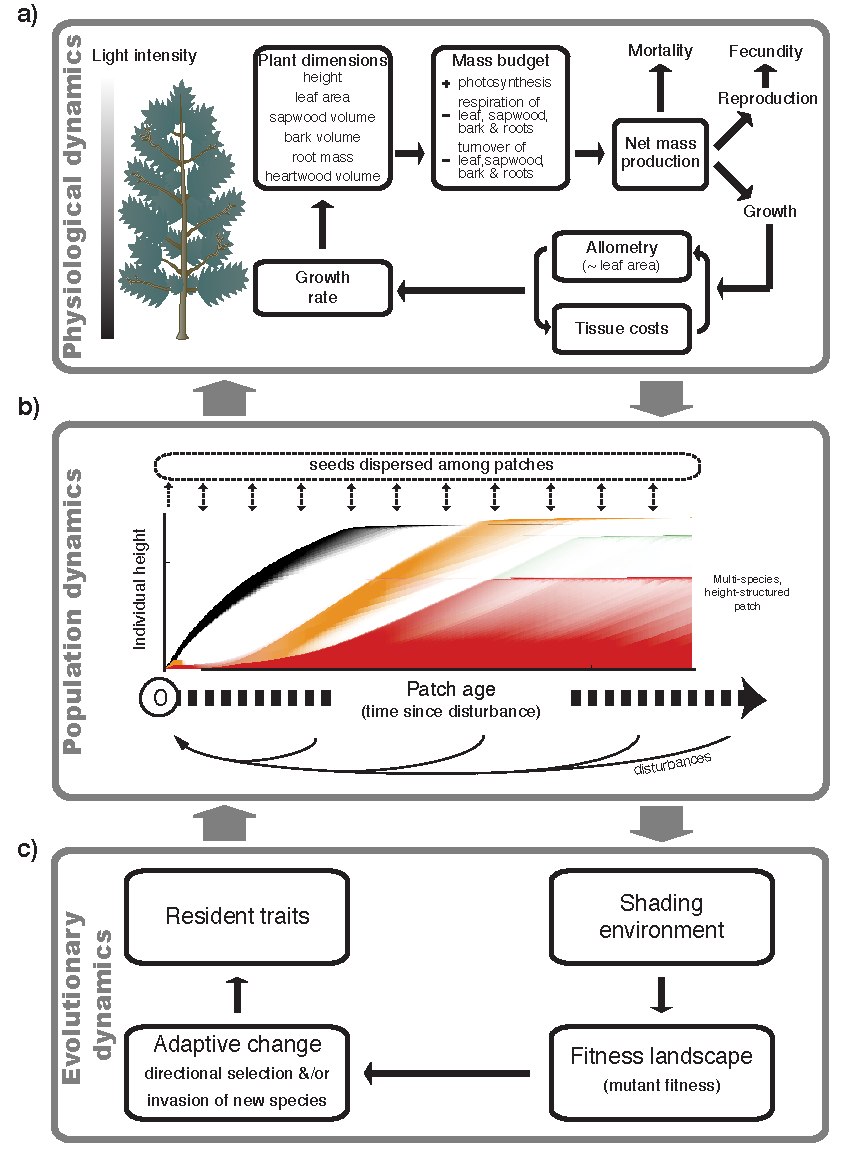
\includegraphics[width=15cm,height=15cm,keepaspectratio]{figures/schematic}

\caption{Processes modelled within {\plant} include physiological, population and
evolutionary dynamics.
Dynamics across all three levels are driven by the
physiological sub-model determining an individual's physiological and
demographic rates on the basis of its traits, size and light environment (a).
(b) Competitive hierarchies  are modelled by tracking the height distribution of
individuals within a ``patch''. The intensity
of shading indicates the density of individuals at a given height for
different species (distinguished by colours). A size- and patch-structured
metapopulation consists of a distribution of patches linked by seed dispersal.
Disturbances occasionally remove all vegetation within a patch, resetting the
patch. (c) The traits of the resident species determine the shading environment
across the metapopulation, which in turn determines the fitness landscape.
Resident traits adjust through directional selection
and through the introduction of new species. Adapted from
\citet{Falster-2011}, \citet{Falster-2015}. }

\label{fig:schematic}
\end{figure}

\newpage

\begin{figure}[h!]
\centering
\includegraphics[width=15cm,height=15cm,keepaspectratio]{figures/plant.pdf}
\caption{Physiological dynamics for individual plants varying in size,
  trait and light environment. Solid lines are for the high
  \textsc{lma} (leaf mass per unit area) strategy, dashed lines are
  for the low \textsc{lma} strategy.  (a) Growth trajectories are
  influenced by both light environment and traits.  (b) Over time, the
  fraction of living tissue switches from leaf towards sapwood, with
  high \textsc{lma} species having relatively more mass in leaf than
  low \textsc{lma} species, due to their longer leaf lifespan. (c) Size-dependent growth rates
  (derivative of panel (a)) peak at around 5m high, but location of the peak
  varies with both trait and light level.  (d) Declines in growth rate
  with light vary with plant size and traits.  Whole plant light
  compensation points (indicated by dots) emerge as the point where
  growth rate is zero (x intercept).  The light level used in panels
  (a) and (c) is indicated with coloured ticks.  See Appendix
  \ref{sec:plant} for further details and code.}
\label{fig:plant}
\end{figure}

\newpage

\begin{figure}[h!]
\centering
\includegraphics[width=15cm,height=15cm,keepaspectratio]{figures/patch.pdf}
\caption{Population dynamics for two species competing within a patch.
  Red and blue lines are low and high \textsc{lma} species from
  Fig. \ref{fig:plant}.  Lines in panel (a) show growth trajectories
  for individuals on the boundary of successive ``cohorts'' for each
  species, using a schedule of introduction times generated by
  {\plant}'s adaptive algorithm.  The initial growth rate advantage of
  the low \textsc{lma} species (see Figure \ref{fig:plant}c) means it
  quickly overtops the high \textsc{lma} species, suppressing its
  growth.  Self-thinning creates space for the high \textsc{lma}
  species to establish below the canopy of the faster species. Panel
  (b) shows the same trajectories as in panel (a), but with shading
  indicating the density $N$ of individuals at given size and patch
  age (light = low density, dark = high density).  (c) The leaf area
  index at ground level for each species.  The dotted line is the
  total leaf area index (summed across both species), and the lines on
  the right side are averages when integrated over the whole
  metapopulation structure.  See Appendix \ref{sec:patch} for further
  details and code.}
\label{fig:patch}
\end{figure}

\newpage

\begin{figure}[h!]
\centering
\includegraphics[width=15cm,height=15cm,keepaspectratio]{figures/emergent.pdf}
\caption{Emergent size-distributions and demography across a metapopulation.
Grey lines show patterns within individual patches differing in time
since disturbance (age), with blue lines indicating patches of a
specific age. Red lines show average relationship across the metapopulation,
obtained by weighting the grey lines by patch and individual abundance.
Panels show (a) patterns of abundance, (b) leaf area and
(c) height growth rate against size. Units of panels (a) and
(b) are amount per unit height per unit ground area.
See Appendix \ref{sec:emergent} for further details and code.}
\label{fig:emergent}
\end{figure}

\newpage

\begin{figure}[h!]
\centering
\includegraphics[width=15cm,height=15cm,keepaspectratio]{figures/fitness.pdf}
\caption{Example fitness landscape for \textsc{lma} (leaf mass per
  unit leaf area), showing potential for stable coexistence of
  multiple types.  Fitness is the log of the population growth rate --
  at zero species are at equilibrium, above zero they will increase in
  density.  (a) Landscape generated by a single species (indicated by
  dots).  At \textsc{lma} of 0.1 (the dashed line, open dot) there is
  directional selection for smaller \textsc{lma}.  At \textsc{lma} of
  0.08 (solid line, filled dot) there is a branching point (see inset
  for more detail).  (b) Landscape generated by two species, holding
  the first at \textsc{lma} of 0.08.  Introducing a species at the
  maximum fitness value from panel (a) reduces the region of positive
  fitness considerably (dashed line, open dot).  Dotted lines show
  subsequent invasions and replacements of the second species, the
  solid line shows a stable fitness landscape where both species exist
  on a peak in the fitness landscape.  At this point no further
  invasion is possible.  See Appendix \ref{sec:fitness} for further
  details and code.}
\label{fig:fitness}
\end{figure}

\clearpage
\setcounter{secnumdepth}{1}

\begin{appendices}\label{sec:appendices}

\section{Plant physiological model}\label{sec:FFW16}

See attached file \url{vignettes/physiology.pdf}

\section{Modelling demography of plants, patches and metapopulations}\label{sec:demography}

See attached file \url{vignettes/demography.pdf}

\section{Plant level properties}\label{sec:plant}

\emph{Note}: due to Manuscript Central not accepting \textsc{html}
files, we have had to convert this (and the following appendices) to
\textsc{pdf}s.  \textsc{html} versions are available on the wiki:
https://github.com/traitecoevo/plant\_paper/wiki --- the \textsc{html}
versions have less pixelated graphics and are easier to copy and
paste out of.

See attached file \url{vignettes/plant.pdf},
source:
\smurl{https://github.com/traitecoevo/plant\_paper/blob/master/vignettes/src/plant.R}
html: \smurl{https://github.com/traitecoevo/plant\_paper/wiki/plant}

\section{Cohort spacing algorithm}\label{sec:cohort-spacing}

See attached file \url{vignettes/cohort_spacing.pdf},
source:
\smurl{https://github.com/traitecoevo/plant\_paper/blob/master/vignettes/src/cohort_spacing.R}
html: \smurl{https://github.com/traitecoevo/plant\_paper/wiki/cohort_spacing}

\section{Finding demographic equilibrium}\label{sec:equilibrium}

See attached file \url{vignettes/equilibrium.pdf}
source:
\smurl{https://github.com/traitecoevo/plant\_paper/blob/master/vignettes/src/equilibrium.R}
html: \smurl{https://github.com/traitecoevo/plant\_paper/wiki/equilibrium}

\section{Patch level dynamics}\label{sec:patch}

See attached file \url{vignettes/patch.pdf}
source:
\smurl{https://github.com/traitecoevo/plant\_paper/blob/master/vignettes/src/patch.R}
html: \smurl{https://github.com/traitecoevo/plant\_paper/wiki/patch}

\section{Patch level emergent properties}\label{sec:emergent}

See attached file \url{vignettes/emergent.pdf}
source:
\smurl{https://github.com/traitecoevo/plant\_paper/blob/master/vignettes/src/emergent.R}
html: \smurl{https://github.com/traitecoevo/plant\_paper/wiki/emergent}

\section{Calculating fitness}\label{sec:fitness}

See attached file \url{vignettes/fitness.pdf}
source:
\smurl{https://github.com/traitecoevo/plant\_paper/blob/master/vignettes/src/fitness.R}
html: \smurl{https://github.com/traitecoevo/plant\_paper/wiki/fitness}

\section{Modifying parameters of the physiological model}\label{sec:parameters}
See attached file \url{vignettes/parameters.pdf}
source:
\smurl{https://github.com/traitecoevo/plant\_paper/blob/master/vignettes/src/parameters.R}
html: \smurl{https://github.com/traitecoevo/plant\_paper/wiki/parameters}

\end{appendices}
\end{document}

%%% Local Variables:
%%% mode: latex
%%% TeX-master: t
%%% TeX-PDF-mode: t
%%% End:

%  LocalWords:  Westoby photosynthate Givnish Enquist Ruger feedbacks
%  LocalWords:  ontogenetic Shugart Tilman Geritz Hubbell Calcagno BH
%  LocalWords:  Cramer Sitch Dekauwe focussed successional Haxeltine
%  LocalWords:  Moorcroft lpj FFW lma wplcp Baltzer Lusk Kohyama pde
%  LocalWords:  Deroos Pacala Strigul ebt adaptively Coomes Binkley
%  LocalWords:  Ogawa Bormann Gyllenberg Vonfoerster Metz Dieckmann
%  LocalWords:  Rcpp Eddelbuettel templated RcppR testhat Wickham DS
%  LocalWords:  Schaling RG Brn nnstr Camac De Roos Duursma Johansson
%  LocalWords:  knitr
